\documentclass[11pt]{article}

\usepackage[margin=1in]{geometry}
\usepackage{graphicx}
\usepackage{array}
\usepackage{longtable}
\usepackage{hyperref}
\usepackage{booktabs}
\usepackage{xcolor}
\usepackage{tikz}
\usepackage{float}
\usepackage{enumitem}
\usepackage{fancyhdr}
\usepackage{titlesec}
\usepackage{tcolorbox}
\usepackage{tabularx}
\usepackage{multirow}
\usepackage{caption}
\usepackage{subcaption}
\usepackage{listings}
\usepackage{pdflscape}
\usepackage{makecell}

\usetikzlibrary{shapes.geometric, arrows.meta, positioning, fit, backgrounds, calc, decorations.pathreplacing}

% Color definitions
\definecolor{componentcolor}{RGB}{70,130,180}
\definecolor{modulecolor}{RGB}{60,179,113}
\definecolor{servicecolor}{RGB}{255,165,0}
\definecolor{datacolor}{RGB}{186,85,211}
\definecolor{flowcolor}{RGB}{100,100,100}
\definecolor{sectionblue}{RGB}{31,78,121}
\definecolor{lightgray}{RGB}{245,245,245}
\definecolor{warningred}{RGB}{220,53,69}
\definecolor{successgreen}{RGB}{40,167,69}
\definecolor{infoblue}{RGB}{23,162,184}
\definecolor{criticalred}{RGB}{200,35,51}
\definecolor{highyellow}{RGB}{255,193,7}
\definecolor{mediumblue}{RGB}{0,123,255}
\definecolor{lowgray}{RGB}{108,117,125}

% Hyperref setup
\hypersetup{
    colorlinks=true,
    linkcolor=sectionblue,
    urlcolor=sectionblue,
    citecolor=sectionblue
}

% Header and footer
\pagestyle{fancy}
\fancyhf{}
\fancyhead[L]{\leftmark}
\fancyhead[R]{Element Catalog Documentation}
\fancyfoot[C]{\thepage}
\renewcommand{\headrulewidth}{0.4pt}
\renewcommand{\footrulewidth}{0.4pt}

% Section formatting
\titleformat{\section}
  {\normalfont\Large\bfseries\color{sectionblue}}{\thesection}{1em}{}
\titleformat{\subsection}
  {\normalfont\large\bfseries\color{sectionblue!80}}{\thesubsection}{1em}{}
\titleformat{\subsubsection}
  {\normalfont\normalsize\bfseries\color{sectionblue!60}}{\thesubsubsection}{1em}{}

% Custom box environments
\newtcolorbox{keypoint}{
    colback=blue!5,
    colframe=sectionblue,
    title=Key Point,
    fonttitle=\bfseries
}

\newtcolorbox{warning}{
    colback=red!5,
    colframe=warningred,
    title=Warning,
    fonttitle=\bfseries
}

\newtcolorbox{bestpractice}{
    colback=green!5,
    colframe=successgreen,
    title=Best Practice,
    fonttitle=\bfseries
}

\newtcolorbox{example}{
    colback=lightgray,
    colframe=flowcolor,
    title=Example,
    fonttitle=\bfseries
}

\newtcolorbox{definition}{
    colback=infoblue!10,
    colframe=infoblue,
    title=Definition,
    fonttitle=\bfseries
}

\newtcolorbox{template}{
    colback=white,
    colframe=flowcolor,
    title=Template,
    fonttitle=\bfseries
}

% Code listing style
\lstset{
    basicstyle=\ttfamily\small,
    breaklines=true,
    frame=single,
    backgroundcolor=\color{lightgray},
    keywordstyle=\color{sectionblue},
    commentstyle=\color{successgreen},
    stringstyle=\color{servicecolor}
}

% Custom column types
\newcolumntype{L}[1]{>{\raggedright\arraybackslash}p{#1}}
\newcolumntype{C}[1]{>{\centering\arraybackslash}p{#1}}
\newcolumntype{R}[1]{>{\raggedleft\arraybackslash}p{#1}}

\title{%
    \vspace{-1cm}
    \textbf{\Huge Software Architecture Documentation}\\[12pt]
    \Large Element Catalog\\[8pt]
    \large A Comprehensive Guide to Documenting Architectural\\
    Elements, Relations, Interfaces, and Behaviors
}
\author{%
    \textit{Architecture Documentation Series}\\[4pt]
    \small Based on SEI Views and Beyond, IEEE 42010, and Industry Best Practices
}
\date{\today}

\begin{document}

\maketitle
\thispagestyle{empty}

\vspace{1cm}

\begin{abstract}
\noindent
The Element Catalog is a critical supporting document that provides detailed specifications for architectural elements depicted in primary architectural views. While diagrams communicate structure and relationships visually, the element catalog captures the rich detail necessary for implementation, analysis, and governance: element properties, interface specifications, behavioral contracts, quality attribute requirements, and traceability information. This comprehensive guide establishes standards and best practices for creating element catalogs that serve as authoritative references throughout the software development lifecycle. The document covers element classification taxonomies, property specification frameworks, relationship documentation patterns, interface contracts, behavioral modeling, and governance processes for maintaining catalog accuracy over time.
\end{abstract}

\vfill

\begin{center}
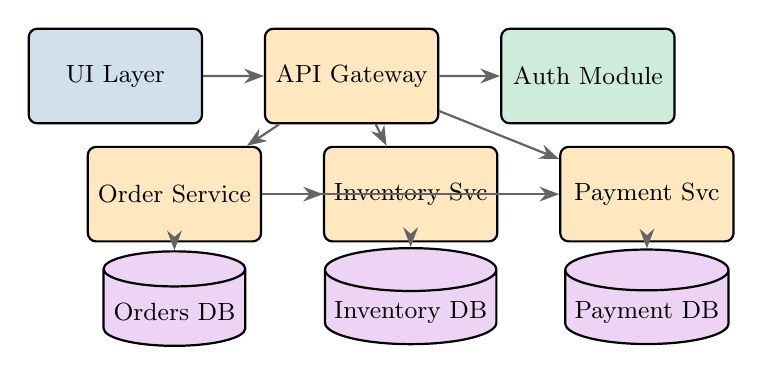
\begin{tikzpicture}[
    scale=0.75,
    component/.style={draw, thick, fill=componentcolor!25, minimum width=2.2cm, minimum height=1.2cm, rounded corners=3pt, font=\small},
    module/.style={draw, thick, fill=modulecolor!25, minimum width=2.2cm, minimum height=1.2cm, rounded corners=3pt, font=\small},
    service/.style={draw, thick, fill=servicecolor!25, minimum width=2.2cm, minimum height=1.2cm, rounded corners=3pt, font=\small},
    data/.style={draw, thick, fill=datacolor!25, cylinder, shape border rotate=90, aspect=0.25, minimum width=1.8cm, minimum height=1.2cm, font=\small},
    flow/.style={-{Stealth[length=2.5mm]}, thick, flowcolor}
]
    % Components
    \node[component] (ui) at (-4,2) {UI Layer};
    \node[service] (api) at (0,2) {API Gateway};
    \node[module] (auth) at (4,2) {Auth Module};
    
    \node[service] (order) at (-3,0) {Order Service};
    \node[service] (inventory) at (1,0) {Inventory Svc};
    \node[service] (payment) at (5,0) {Payment Svc};
    
    \node[data] (orderdb) at (-3,-2) {Orders DB};
    \node[data] (invdb) at (1,-2) {Inventory DB};
    \node[data] (paydb) at (5,-2) {Payment DB};
    
    % Flows
    \draw[flow] (ui) -- (api);
    \draw[flow] (api) -- (auth);
    \draw[flow] (api) -- (order);
    \draw[flow] (api) -- (inventory);
    \draw[flow] (api) -- (payment);
    \draw[flow] (order) -- (orderdb);
    \draw[flow] (inventory) -- (invdb);
    \draw[flow] (payment) -- (paydb);
    \draw[flow] (order) -- (inventory);
    \draw[flow] (order) -- (payment);
\end{tikzpicture}
\end{center}

\newpage
\tableofcontents
\newpage

%==============================================================================
\section{Introduction to the Element Catalog}
%==============================================================================

\subsection{Definition and Purpose}

The Element Catalog is a structured repository of detailed information about architectural elements and their relationships within a specific architectural view. While primary view presentations (diagrams) communicate structure visually, they cannot convey the depth of information necessary for implementation, analysis, and maintenance. The element catalog bridges this gap by providing comprehensive specifications in a consistent, searchable format.

\begin{definition}
An \textbf{Element Catalog} is a supplementary documentation artifact that records detailed properties, interfaces, behaviors, and relationships for each element appearing in an architectural view, providing the authoritative reference for understanding element specifications and contracts.
\end{definition}

The element catalog serves several critical purposes. First, it provides \textbf{complete specification} by capturing information that cannot be represented in diagrams, including detailed properties, interface contracts, behavioral constraints, and quality requirements. Second, it enables \textbf{analysis support} by providing the data necessary for architectural analysis, including dependency analysis, impact assessment, and quality attribute evaluation. Third, it facilitates \textbf{implementation guidance} by giving developers precise specifications for implementing, integrating, and testing architectural elements. Fourth, it supports \textbf{governance} by establishing the authoritative source for architectural decisions, enabling conformance checking and change impact analysis. Fifth, it enables \textbf{knowledge preservation} by documenting institutional knowledge about element purposes, constraints, and evolution history.

\subsection{Relationship to Architectural Views}

The element catalog has an intimate relationship with the architectural view it supplements. Every element appearing in a view's primary presentation should have a corresponding entry in the catalog. The view diagram and catalog together form a complete architectural view.

\begin{figure}[H]
\centering
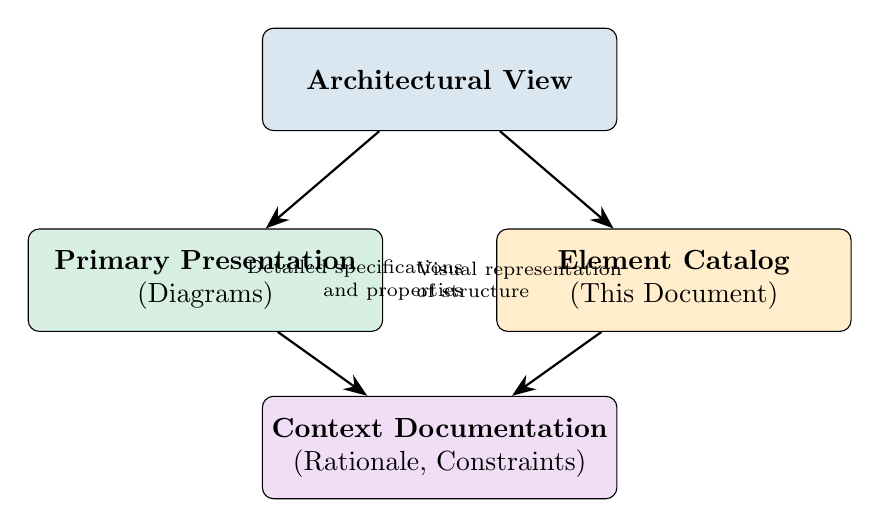
\begin{tikzpicture}[
    scale=0.85,
    box/.style={draw, rounded corners, minimum width=4.5cm, minimum height=1.3cm, align=center},
    arrow/.style={-{Stealth[length=3mm]}, thick}
]
    \node[box, fill=componentcolor!20] (view) at (0,3) {\textbf{Architectural View}};
    \node[box, fill=modulecolor!20] (primary) at (-3.5,0) {\textbf{Primary Presentation}\\(Diagrams)};
    \node[box, fill=servicecolor!20] (catalog) at (3.5,0) {\textbf{Element Catalog}\\(This Document)};
    \node[box, fill=datacolor!20] (context) at (0,-2.5) {\textbf{Context Documentation}\\(Rationale, Constraints)};
    
    \draw[arrow] (view) -- (primary);
    \draw[arrow] (view) -- (catalog);
    \draw[arrow] (primary) -- (context);
    \draw[arrow] (catalog) -- (context);
    
    \node[right=0.3cm of primary, text width=3cm, font=\scriptsize, align=left] {Visual representation\\of structure};
    \node[left=0.3cm of catalog, text width=3cm, font=\scriptsize, align=right] {Detailed specifications\\and properties};
\end{tikzpicture}
\caption{Element Catalog within Architectural View Structure}
\end{figure}

The catalog complements the primary presentation by providing depth where the diagram provides breadth. A well-designed diagram shows the ``what'' and ``how'' of structure at a glance; the catalog explains the ``why'' and provides the detail necessary for implementation.

\subsection{Catalog Scope and Boundaries}

Each element catalog is scoped to a specific architectural view. A system with multiple views (module view, component-and-connector view, deployment view) will have multiple element catalogs, each documenting elements appropriate to that view's concerns.

The catalog scope should align with the view scope. For a module decomposition view, the catalog documents modules and their decomposition relationships. For a client-server view, the catalog documents clients, servers, and their interaction protocols. For a deployment view, the catalog documents deployment nodes and artifact mappings.

\begin{keypoint}
Maintain a one-to-one correspondence between architectural views and element catalogs. Each view has exactly one catalog, and each catalog documents exactly one view. Cross-view relationships should be captured through explicit traceability references rather than duplicating element definitions.
\end{keypoint}

\subsection{Standards and Frameworks}

The element catalog concept derives from several architectural documentation standards. The SEI ``Views and Beyond'' approach explicitly defines the element catalog as a required component of every architectural view. IEEE 42010 (Systems and Software Engineering---Architecture Description) establishes the framework for architectural views and viewpoints that catalogs support. ISO/IEC 25010 provides the quality model that informs element quality attribute documentation. ArchiMate provides element taxonomies applicable to enterprise architecture catalogs. The C4 Model defines element hierarchies (System, Container, Component) that inform catalog structure.

%==============================================================================
\section{How to Read and Use This Catalog}
%==============================================================================

\subsection{Catalog Organization}

This element catalog is organized into four major sections that progressively build understanding of the architectural elements. Section A (Elements and Properties) documents each element's identity, purpose, responsibilities, and key properties. Section B (Relations and Properties) captures the relationships among elements, including their types, directions, and quality requirements. Section C (Element Interfaces) specifies the externally visible contracts through which elements interact. Section D (Element Behavior) describes dynamic aspects including state machines, lifecycle events, and algorithmic responsibilities.

Each section uses consistent formatting and conventions described in this chapter. Readers should familiarize themselves with these conventions before diving into the detailed specifications.

\subsection{Naming Conventions}

Consistent naming enables efficient navigation and cross-referencing. This catalog uses the following naming conventions.

For \textbf{element identifiers}, the format is \texttt{<Type>-<Domain>-<Name>-<Version>}. The type prefix indicates the element kind (SVC for service, MOD for module, CMP for component, DAT for data store). The domain indicates the functional area. The name is a descriptive identifier. The version is optional for versioned elements. Examples include \texttt{SVC-ORDER-Processing-v2}, \texttt{MOD-AUTH-TokenValidator}, and \texttt{CMP-UI-ShoppingCart}.

For \textbf{interface identifiers}, the format is \texttt{<Element>.<Interface>}. Examples include \texttt{SVC-ORDER-Processing.CreateOrder} and \texttt{MOD-AUTH-TokenValidator.ValidateToken}.

For \textbf{relation identifiers}, the format is \texttt{REL-<Source>-<Target>-<Type>}. Examples include \texttt{REL-OrderSvc-InventorySvc-Calls} and \texttt{REL-WebApp-AuthMod-DependsOn}.

\subsection{Cross-Reference Notation}

Cross-references to other documents, views, and artifacts use the following notation. References to other views appear as \texttt{[VIEW:<ViewName>]}, such as \texttt{[VIEW:Deployment]} or \texttt{[VIEW:ModuleDecomposition]}. References to requirements appear as \texttt{[REQ:<RequirementID>]}, such as \texttt{[REQ:FR-101]} or \texttt{[REQ:NFR-PERF-03]}. References to implementation artifacts appear as \texttt{[IMPL:<ArtifactPath>]}, such as \texttt{[IMPL:src/services/order/]}. References to external documentation appear as \texttt{[DOC:<DocumentID>]}, such as \texttt{[DOC:API-Spec-v2.1]}.

\subsection{Property Value Conventions}

Properties throughout the catalog use standardized value formats. Criticality levels use \textbf{Critical} (system failure if unavailable), \textbf{High} (significant degradation if unavailable), \textbf{Medium} (partial functionality affected), and \textbf{Low} (minimal impact if unavailable). Availability targets use percentage notation such as 99.99\%, 99.9\%, or 99\%. Latency requirements use millisecond notation such as $<$50ms, $<$200ms, or $<$1s. Throughput requirements use rate notation such as 1000 req/s, 10K msg/min, or 1M records/day. Data volumes use standard units such as GB, TB, or records/day.

\subsection{Reading Strategies}

Different readers will approach this catalog with different goals. Developers implementing a specific element should start with that element's entry in Section A, review its interfaces in Section C, and understand its behavioral contracts in Section D. Integration engineers should focus on Section B (Relations) and Section C (Interfaces) to understand how elements connect. Architects performing analysis should review all sections, paying particular attention to criticality ratings, quality requirements, and dependency patterns. Operators should focus on criticality, availability targets, and behavioral aspects related to operational concerns.

%==============================================================================
\section{Element Classification and Taxonomy}
%==============================================================================

\subsection{Element Type Hierarchy}

Architectural elements can be classified into a taxonomy that aids understanding and enables consistent documentation. The following hierarchy provides a comprehensive classification scheme.

\begin{figure}[H]
\centering
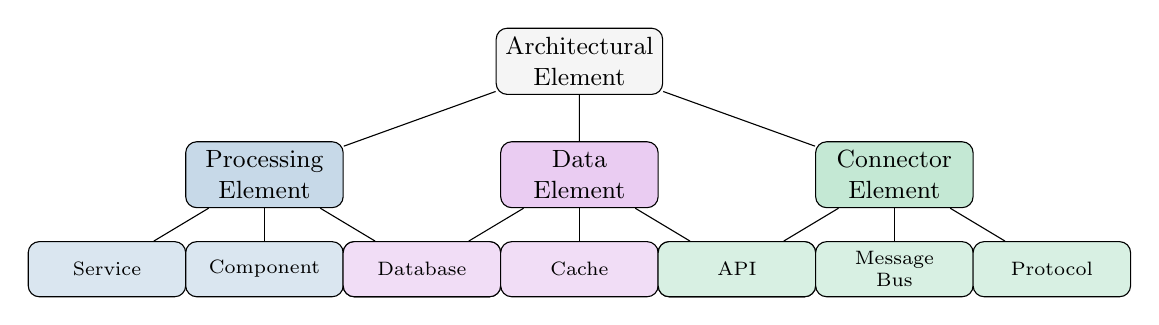
\begin{tikzpicture}[
    scale=0.8,
    level 1/.style={sibling distance=5cm, level distance=1.8cm},
    level 2/.style={sibling distance=2.5cm, level distance=1.5cm},
    every node/.style={draw, rounded corners, minimum width=2cm, minimum height=0.7cm, font=\small, align=center}
]
    \node[fill=lightgray] {Architectural\\Element}
        child {node[fill=componentcolor!30] {Processing\\Element}
            child {node[fill=componentcolor!20, font=\scriptsize] {Service}}
            child {node[fill=componentcolor!20, font=\scriptsize] {Component}}
            child {node[fill=componentcolor!20, font=\scriptsize] {Module}}
        }
        child {node[fill=datacolor!30] {Data\\Element}
            child {node[fill=datacolor!20, font=\scriptsize] {Database}}
            child {node[fill=datacolor!20, font=\scriptsize] {Cache}}
            child {node[fill=datacolor!20, font=\scriptsize] {Queue}}
        }
        child {node[fill=modulecolor!30] {Connector\\Element}
            child {node[fill=modulecolor!20, font=\scriptsize] {API}}
            child {node[fill=modulecolor!20, font=\scriptsize] {Message\\Bus}}
            child {node[fill=modulecolor!20, font=\scriptsize] {Protocol}}
        };
\end{tikzpicture}
\caption{Element Type Taxonomy}
\end{figure}

\subsubsection{Processing Elements}

Processing elements perform computation, transformation, or coordination. \textbf{Services} are independently deployable units providing business capabilities through well-defined interfaces, typically in service-oriented or microservices architectures. \textbf{Components} are modular units of functionality with explicit interfaces, deployable as part of a larger application. \textbf{Modules} are logical groupings of code organized by responsibility or domain, representing compile-time structure. \textbf{Functions} are discrete units of computation, particularly relevant in serverless architectures. \textbf{Processes} are runtime execution units that may contain multiple threads or components.

\subsubsection{Data Elements}

Data elements store, manage, or transport information. \textbf{Databases} provide persistent storage with query capabilities, including relational, document, graph, and time-series variants. \textbf{Caches} provide high-speed temporary storage for frequently accessed data. \textbf{Message Queues} provide asynchronous message storage and delivery. \textbf{File Stores} provide unstructured or semi-structured data storage. \textbf{Data Streams} provide continuous data flow for real-time processing.

\subsubsection{Connector Elements}

Connector elements facilitate interaction between other elements. \textbf{APIs} define synchronous request-response interfaces. \textbf{Message Buses} provide publish-subscribe or point-to-point asynchronous messaging. \textbf{Event Brokers} manage event distribution and subscription. \textbf{Load Balancers} distribute requests across multiple instances. \textbf{Service Meshes} provide inter-service communication infrastructure.

\subsection{View-Specific Element Types}

Different architectural views emphasize different element types. The following table maps common views to their typical element types.

\begin{longtable}{@{}L{3.5cm} L{4cm} L{5.5cm}@{}}
\caption{View-Specific Element Types} \\
\toprule
\textbf{Architectural View} & \textbf{Primary Elements} & \textbf{Primary Relations} \\
\midrule
\endfirsthead
\toprule
\textbf{Architectural View} & \textbf{Primary Elements} & \textbf{Primary Relations} \\
\midrule
\endhead
\midrule
\multicolumn{3}{r}{\textit{Continued on next page}} \\
\endfoot
\bottomrule
\endlastfoot
Module Decomposition & Modules, Packages, Classes & Contains, Uses, Depends-on \\
Component-Connector & Components, Connectors, Ports & Attaches, Connects, Flows-to \\
Client-Server & Clients, Servers, Tiers & Requests, Responds, Invokes \\
Service-Oriented & Services, Endpoints, Contracts & Calls, Publishes, Subscribes \\
Deployment & Nodes, Artifacts, Environments & Deploys-to, Hosts, Manifests \\
Data Flow & Processes, Data Stores, Flows & Reads, Writes, Transforms \\
Layered & Layers, Modules within Layers & Uses (constrained by layer rules) \\
Microservices & Services, APIs, Data Stores & Calls, Events, Sagas \\
\end{longtable}

\subsection{Element Stereotypes}

Within each element type, stereotypes provide additional classification. Stereotypes communicate patterns, roles, or implementation guidance.

\begin{example}
\textbf{Service Stereotypes:}
\begin{itemize}[nosep]
    \item \texttt{<<aggregate-root>>} -- Service managing a DDD aggregate
    \item \texttt{<<gateway>>} -- Entry point service handling cross-cutting concerns
    \item \texttt{<<orchestrator>>} -- Service coordinating multi-step workflows
    \item \texttt{<<adapter>>} -- Service adapting external system interfaces
    \item \texttt{<<facade>>} -- Service simplifying complex subsystem access
\end{itemize}

\textbf{Data Store Stereotypes:}
\begin{itemize}[nosep]
    \item \texttt{<<system-of-record>>} -- Authoritative source for specific data
    \item \texttt{<<read-replica>>} -- Read-optimized copy of data
    \item \texttt{<<event-store>>} -- Append-only event persistence
    \item \texttt{<<cache>>} -- Temporary high-speed storage
\end{itemize}
\end{example}

%==============================================================================
\section{Section A: Elements and Their Properties}
%==============================================================================

\subsection{Element Documentation Framework}

Each element in the catalog receives comprehensive documentation following a consistent framework. This framework ensures that all information necessary for understanding, implementing, and maintaining the element is captured systematically.

\begin{template}
\textbf{Element Specification Template}

\vspace{0.3cm}
\textbf{Element Identity}
\begin{itemize}[nosep]
    \item \textbf{ID:} Unique identifier following naming conventions
    \item \textbf{Name:} Human-readable name
    \item \textbf{Type:} Classification from taxonomy
    \item \textbf{Stereotype:} Optional pattern or role indicator
    \item \textbf{Version:} Current version number
\end{itemize}

\vspace{0.2cm}
\textbf{Description and Responsibility}
\begin{itemize}[nosep]
    \item \textbf{Purpose:} Why this element exists
    \item \textbf{Responsibilities:} What this element does (and does not do)
    \item \textbf{Domain:} Business or technical domain
\end{itemize}

\vspace{0.2cm}
\textbf{Properties}
\begin{itemize}[nosep]
    \item \textbf{Criticality:} Impact of failure
    \item \textbf{Quality Attributes:} Performance, availability, security requirements
    \item \textbf{Technology Stack:} Implementation technologies
    \item \textbf{Constraints:} Limitations and restrictions
\end{itemize}

\vspace{0.2cm}
\textbf{Traceability}
\begin{itemize}[nosep]
    \item \textbf{Requirements:} Linked requirements
    \item \textbf{Implementation:} Source code or artifact references
    \item \textbf{Related Views:} Appearances in other views
\end{itemize}
\end{template}

\subsection{Identity Properties}

Identity properties uniquely identify and classify the element.

\subsubsection{Element Identifier}

The element identifier (ID) must be globally unique within the architecture and stable across versions. IDs should be meaningful (conveying type and purpose) yet concise. Once assigned, IDs should not change; if an element is fundamentally redesigned, it should receive a new ID.

\subsubsection{Versioning}

Elements evolve over time. The catalog should track version information including the current version number (following semantic versioning where applicable), version history summary, compatibility notes (backward/forward compatibility with previous versions), and deprecation status if applicable.

\begin{longtable}{@{}L{2cm} L{2.5cm} L{3.5cm} L{4.5cm}@{}}
\caption{Element Version History Example} \\
\toprule
\textbf{Version} & \textbf{Date} & \textbf{Changes} & \textbf{Compatibility} \\
\midrule
\endfirsthead
\toprule
\textbf{Version} & \textbf{Date} & \textbf{Changes} & \textbf{Compatibility} \\
\midrule
\endhead
\bottomrule
\endlastfoot
1.0.0 & 2024-01-15 & Initial release & N/A \\
1.1.0 & 2024-03-20 & Added batch processing capability & Backward compatible \\
2.0.0 & 2024-06-01 & Redesigned API; new data model & Breaking changes; migration required \\
2.0.1 & 2024-06-15 & Bug fixes for edge cases & Fully compatible with 2.0.0 \\
\end{longtable}

\subsection{Description and Responsibilities}

The description section captures the element's purpose and scope through several components.

\subsubsection{Purpose Statement}

The purpose statement explains why the element exists---what problem it solves or what value it provides. A good purpose statement is concise (1-3 sentences), business-oriented (explaining value, not just function), and unique (distinguishing this element from others).

\begin{example}
\textbf{Good Purpose Statement:}
``The Order Processing Service validates customer orders, coordinates inventory reservation, and initiates payment processing to enable reliable order fulfillment within the e-commerce platform.''

\textbf{Poor Purpose Statement:}
``This service processes orders.'' (Too vague, doesn't explain value or distinguish from other services)
\end{example}

\subsubsection{Responsibilities}

Responsibilities define what the element does and, importantly, what it does not do. Following the Single Responsibility Principle, each element should have a cohesive set of responsibilities. Document responsibilities as a list of specific duties. Include explicit non-responsibilities to prevent scope creep. Explain the rationale for responsibility boundaries.

\begin{example}
\textbf{Order Processing Service Responsibilities:}
\begin{itemize}[nosep]
    \item Validate order requests against business rules
    \item Calculate order totals including taxes and discounts
    \item Coordinate with Inventory Service to reserve stock
    \item Initiate payment processing via Payment Service
    \item Persist order records to Order Database
    \item Publish order events for downstream processing
\end{itemize}

\textbf{Non-Responsibilities (handled by other elements):}
\begin{itemize}[nosep]
    \item Inventory management (Inventory Service)
    \item Payment processing logic (Payment Service)
    \item Shipping logistics (Fulfillment Service)
    \item Customer notifications (Notification Service)
\end{itemize}
\end{example}

\subsection{Element Properties}

Properties capture measurable or classifiable characteristics of the element.

\subsubsection{Criticality Assessment}

Criticality indicates the business impact of element failure. Use a consistent scale across all elements.

\begin{longtable}{@{}L{2cm} L{3cm} L{4cm} L{3.5cm}@{}}
\caption{Criticality Classification Scale} \\
\toprule
\textbf{Level} & \textbf{Business Impact} & \textbf{Example Consequences} & \textbf{Response} \\
\midrule
\endfirsthead
\toprule
\textbf{Level} & \textbf{Business Impact} & \textbf{Example Consequences} & \textbf{Response} \\
\midrule
\endhead
\bottomrule
\endlastfoot
\cellcolor{criticalred!20}\textbf{Critical} & Complete business stoppage & No orders processed; revenue loss; regulatory violation & Immediate escalation; 24/7 support; redundancy required \\
\cellcolor{highyellow!30}\textbf{High} & Significant degradation & Major features unavailable; customer-facing impact & Urgent response; business hours escalation \\
\cellcolor{mediumblue!20}\textbf{Medium} & Partial functionality loss & Some features degraded; workarounds available & Standard response; next business day \\
\cellcolor{lowgray!20}\textbf{Low} & Minimal impact & Internal tools affected; no customer impact & Scheduled maintenance acceptable \\
\end{longtable}

\subsubsection{Quality Attribute Requirements}

Each element may have specific quality attribute requirements that constrain its design and implementation.

\begin{longtable}{@{}L{2.8cm} L{3cm} L{3.5cm} L{3.2cm}@{}}
\caption{Element Quality Attribute Template} \\
\toprule
\textbf{Attribute} & \textbf{Requirement} & \textbf{Measure} & \textbf{Verification} \\
\midrule
\endfirsthead
\toprule
\textbf{Attribute} & \textbf{Requirement} & \textbf{Measure} & \textbf{Verification} \\
\midrule
\endhead
\bottomrule
\endlastfoot
Performance & Response time & 95th percentile $<$ 200ms & Load testing \\
Availability & Uptime & 99.9\% monthly & Monitoring \\
Scalability & Throughput & 10,000 req/sec at peak & Capacity testing \\
Security & Data protection & PII encrypted at rest/transit & Security audit \\
Reliability & Error rate & $<$ 0.1\% failed requests & Error tracking \\
Maintainability & Code coverage & $>$ 80\% unit test coverage & CI pipeline \\
\end{longtable}

\subsubsection{Technology Stack}

Document the technology choices for each element to support implementation and operational concerns.

\begin{longtable}{@{}L{3cm} L{4cm} L{5.5cm}@{}}
\caption{Technology Stack Documentation} \\
\toprule
\textbf{Category} & \textbf{Technology} & \textbf{Rationale/Notes} \\
\midrule
\endfirsthead
\toprule
\textbf{Category} & \textbf{Technology} & \textbf{Rationale/Notes} \\
\midrule
\endhead
\bottomrule
\endlastfoot
Language & Java 17 & Standard platform; team expertise \\
Framework & Spring Boot 3.x & Mature ecosystem; microservices support \\
Database & PostgreSQL 15 & ACID compliance; complex queries \\
Cache & Redis 7.x & High-performance caching; pub/sub \\
Message Queue & Apache Kafka & Event streaming; high throughput \\
Container Runtime & Docker / Kubernetes & Standard deployment; orchestration \\
Observability & OpenTelemetry, Prometheus & Distributed tracing; metrics \\
\end{longtable}

\subsubsection{Constraints}

Constraints document limitations, restrictions, and assumptions that affect the element.

\begin{itemize}
    \item \textbf{Technical Constraints:} Platform limitations, technology mandates, integration requirements
    \item \textbf{Business Constraints:} Regulatory requirements, licensing restrictions, budget limitations
    \item \textbf{Operational Constraints:} Deployment windows, geographic restrictions, support requirements
    \item \textbf{Design Constraints:} Architectural patterns required, interfaces that must be preserved
\end{itemize}

\subsection{Comprehensive Element Registry}

The element registry provides a summary table of all elements, enabling quick reference and navigation.

\setlength{\extrarowheight}{4pt}
\begin{longtable}{@{}L{2.8cm} L{1.5cm} L{1.3cm} L{2.2cm} L{4.2cm}@{}}
\caption{Element Registry} \\
\toprule
\textbf{Element ID} & \textbf{Type} & \textbf{Critical.} & \textbf{Technology} & \textbf{Primary Responsibility} \\
\midrule
\endfirsthead
\toprule
\textbf{Element ID} & \textbf{Type} & \textbf{Critical.} & \textbf{Technology} & \textbf{Primary Responsibility} \\
\midrule
\endhead
\midrule
\multicolumn{5}{r}{\textit{Continued on next page}} \\
\endfoot
\bottomrule
\endlastfoot
SVC-API-Gateway & Service & Critical & Node.js, Kong & Route requests; authentication; rate limiting \\
SVC-ORDER-Process & Service & Critical & Java, Spring & Order validation, coordination, persistence \\
SVC-INV-Manager & Service & High & Go & Inventory tracking, reservation, alerts \\
SVC-PAY-Process & Service & Critical & Java, Spring & Payment processing, refunds, reconciliation \\
SVC-USER-Auth & Service & Critical & Go, OAuth2 & Authentication, authorization, token management \\
SVC-NOTIFY-Send & Service & Medium & Python & Email, SMS, push notifications \\
DAT-ORDER-DB & Database & Critical & PostgreSQL & Order records, transaction history \\
DAT-INV-DB & Database & High & PostgreSQL & Inventory levels, locations, movements \\
DAT-USER-DB & Database & Critical & PostgreSQL & User accounts, profiles, credentials \\
DAT-CACHE-Redis & Cache & High & Redis & Session data, API responses, rate limits \\
MSG-EVENT-Bus & Queue & High & Kafka & Async event distribution, event sourcing \\
\end{longtable}

\subsection{Detailed Element Specifications}

Following the registry, provide detailed specifications for each element. The following example demonstrates the full documentation format.

\begin{tcolorbox}[colback=lightgray, colframe=sectionblue, title=\textbf{Element: SVC-ORDER-Process}]

\textbf{Identity}
\begin{itemize}[nosep]
    \item \textbf{ID:} SVC-ORDER-Process
    \item \textbf{Name:} Order Processing Service
    \item \textbf{Type:} Service
    \item \textbf{Stereotype:} \texttt{<<orchestrator>>}
    \item \textbf{Version:} 2.3.1
\end{itemize}

\vspace{0.3cm}
\textbf{Purpose}\\
Orchestrates the order lifecycle from submission through fulfillment initiation, ensuring business rules are enforced, inventory is reserved, and payment is processed before committing orders.

\vspace{0.3cm}
\textbf{Responsibilities}
\begin{itemize}[nosep]
    \item Validate order requests against business rules and customer eligibility
    \item Calculate order totals including line items, taxes, discounts, and shipping
    \item Coordinate with Inventory Service to reserve stock (saga participant)
    \item Initiate payment authorization via Payment Service
    \item Persist order records with full audit trail
    \item Publish OrderCreated, OrderUpdated, OrderCancelled events
    \item Handle order modifications and cancellations within policy windows
\end{itemize}

\vspace{0.3cm}
\textbf{Non-Responsibilities}
\begin{itemize}[nosep]
    \item Inventory management and warehouse operations (SVC-INV-Manager)
    \item Payment gateway integration and PCI compliance (SVC-PAY-Process)
    \item Shipping carrier integration (SVC-FULFILL-Ship)
    \item Customer communication (SVC-NOTIFY-Send)
\end{itemize}

\vspace{0.3cm}
\textbf{Properties}
\begin{itemize}[nosep]
    \item \textbf{Criticality:} Critical---order processing is core revenue path
    \item \textbf{Availability Target:} 99.95\% (4.4 hours downtime/year max)
    \item \textbf{Performance:} Order creation $<$ 500ms (95th percentile)
    \item \textbf{Throughput:} 1,000 orders/minute sustained; 5,000/minute peak
    \item \textbf{Data Volume:} ~50KB per order; 2M orders/month
    \item \textbf{Security:} PII handling; SOC 2 compliant
\end{itemize}

\vspace{0.3cm}
\textbf{Technology Stack}
\begin{itemize}[nosep]
    \item Runtime: Java 17 on Spring Boot 3.2
    \item Database: PostgreSQL 15 (primary); Redis (caching)
    \item Messaging: Apache Kafka (event publishing)
    \item Deployment: Kubernetes (3 replicas minimum)
\end{itemize}

\vspace{0.3cm}
\textbf{Constraints}
\begin{itemize}[nosep]
    \item Must maintain backward compatibility with mobile app v3.x
    \item Cannot store payment card numbers (PCI-DSS)
    \item Must support idempotent order creation for retry safety
    \item Geographic data residency: orders from EU stored in EU region
\end{itemize}

\vspace{0.3cm}
\textbf{Traceability}
\begin{itemize}[nosep]
    \item Requirements: [REQ:FR-ORD-001] through [REQ:FR-ORD-050]
    \item Implementation: [IMPL:services/order-service/]
    \item Deployment View: [VIEW:Deployment] Node: order-service-cluster
    \item API Documentation: [DOC:API-Order-v2.3]
\end{itemize}
\end{tcolorbox}

%==============================================================================
\section{Section B: Relations and Their Properties}
%==============================================================================

\subsection{Relationship Type Taxonomy}

Relationships between elements capture how elements interact, depend on, or contain one another. Understanding relationship types is essential for dependency analysis, impact assessment, and implementation planning.

\subsubsection{Structural Relationships}

Structural relationships describe static organization.

\begin{longtable}{@{}L{2.5cm} L{3.5cm} L{6.5cm}@{}}
\caption{Structural Relationship Types} \\
\toprule
\textbf{Relation} & \textbf{Notation} & \textbf{Description} \\
\midrule
\endfirsthead
\toprule
\textbf{Relation} & \textbf{Notation} & \textbf{Description} \\
\midrule
\endhead
\bottomrule
\endlastfoot
Contains & A \texttt{contains} B & A is composed of B; B exists only within A's context \\
Uses & A \texttt{uses} B & A requires B's functionality; compile/build-time dependency \\
Depends-on & A \texttt{depends-on} B & A requires B at runtime; A cannot function without B \\
Extends & A \texttt{extends} B & A specializes or inherits from B \\
Implements & A \texttt{implements} B & A provides concrete realization of B (interface) \\
Aggregates & A \texttt{aggregates} B & A references B; B can exist independently \\
\end{longtable}

\subsubsection{Behavioral Relationships}

Behavioral relationships describe runtime interactions.

\begin{longtable}{@{}L{2.5cm} L{3.5cm} L{6.5cm}@{}}
\caption{Behavioral Relationship Types} \\
\toprule
\textbf{Relation} & \textbf{Notation} & \textbf{Description} \\
\midrule
\endfirsthead
\toprule
\textbf{Relation} & \textbf{Notation} & \textbf{Description} \\
\midrule
\endhead
\bottomrule
\endlastfoot
Calls & A \texttt{calls} B & A invokes B's interface synchronously \\
Sends & A \texttt{sends} B & A transmits message/data to B asynchronously \\
Publishes-to & A \texttt{publishes-to} B & A emits events that B distributes \\
Subscribes-to & A \texttt{subscribes-to} B & A receives events from B \\
Reads-from & A \texttt{reads-from} B & A retrieves data from B (data store) \\
Writes-to & A \texttt{writes-to} B & A persists data to B (data store) \\
Triggers & A \texttt{triggers} B & A causes B to execute (event-driven) \\
\end{longtable}

\subsubsection{Deployment Relationships}

Deployment relationships describe how elements map to infrastructure.

\begin{longtable}{@{}L{2.5cm} L{3.5cm} L{6.5cm}@{}}
\caption{Deployment Relationship Types} \\
\toprule
\textbf{Relation} & \textbf{Notation} & \textbf{Description} \\
\midrule
\endfirsthead
\toprule
\textbf{Relation} & \textbf{Notation} & \textbf{Description} \\
\midrule
\endhead
\bottomrule
\endlastfoot
Deploys-to & A \texttt{deploys-to} B & Artifact A is deployed on node B \\
Runs-on & A \texttt{runs-on} B & Process A executes on platform B \\
Hosts & A \texttt{hosts} B & Node A provides runtime for B \\
Connects-to & A \texttt{connects-to} B & Node A has network path to node B \\
\end{longtable}

\subsection{Relationship Properties}

Each relationship should be documented with properties that enable analysis and implementation.

\begin{template}
\textbf{Relationship Specification Template}

\vspace{0.2cm}
\textbf{Identity}
\begin{itemize}[nosep]
    \item \textbf{ID:} Unique relationship identifier
    \item \textbf{Source:} Originating element
    \item \textbf{Target:} Destination element
    \item \textbf{Type:} Relationship classification
\end{itemize}

\vspace{0.2cm}
\textbf{Interaction Properties}
\begin{itemize}[nosep]
    \item \textbf{Direction:} Unidirectional / Bidirectional
    \item \textbf{Cardinality:} 1:1, 1:N, N:M
    \item \textbf{Timing:} Synchronous / Asynchronous
    \item \textbf{Protocol:} Communication mechanism
    \item \textbf{Data Format:} Message/payload format
\end{itemize}

\vspace{0.2cm}
\textbf{Quality Requirements}
\begin{itemize}[nosep]
    \item \textbf{Latency:} Response time requirement
    \item \textbf{Throughput:} Volume requirement
    \item \textbf{Reliability:} Delivery guarantee
    \item \textbf{Security:} Authentication/encryption
\end{itemize}

\vspace{0.2cm}
\textbf{Failure Handling}
\begin{itemize}[nosep]
    \item \textbf{Timeout:} Maximum wait time
    \item \textbf{Retry Policy:} Retry strategy
    \item \textbf{Fallback:} Degraded behavior
    \item \textbf{Circuit Breaker:} Failure threshold
\end{itemize}
\end{template}

\subsection{Relationship Registry}

The relationship registry provides a comprehensive view of all element relationships.

\setlength{\extrarowheight}{4pt}
\begin{longtable}{@{}L{2.3cm} L{2.3cm} L{1.8cm} L{2cm} L{3.8cm}@{}}
\caption{Relationship Registry} \\
\toprule
\textbf{Source} & \textbf{Target} & \textbf{Type} & \textbf{Protocol} & \textbf{Key Properties} \\
\midrule
\endfirsthead
\toprule
\textbf{Source} & \textbf{Target} & \textbf{Type} & \textbf{Protocol} & \textbf{Key Properties} \\
\midrule
\endhead
\midrule
\multicolumn{5}{r}{\textit{Continued on next page}} \\
\endfoot
\bottomrule
\endlastfoot
API-Gateway & ORDER-Svc & calls & HTTP/REST & Sync; $<$100ms; JWT auth; retry 3x \\
API-Gateway & USER-Auth & calls & HTTP/REST & Sync; $<$50ms; mTLS; critical path \\
ORDER-Svc & INV-Svc & calls & gRPC & Sync; $<$200ms; saga participant \\
ORDER-Svc & PAY-Svc & calls & HTTP/REST & Sync; $<$5s timeout; idempotent \\
ORDER-Svc & ORDER-DB & writes & PostgreSQL & Transactional; ACID; 10K TPS \\
ORDER-Svc & EVENT-Bus & publishes & Kafka & Async; at-least-once; ordered \\
INV-Svc & INV-DB & reads/writes & PostgreSQL & Read replicas; 50K queries/sec \\
INV-Svc & EVENT-Bus & subscribes & Kafka & Consumer group; offset tracking \\
NOTIFY-Svc & EVENT-Bus & subscribes & Kafka & Non-critical; best-effort delivery \\
CACHE-Redis & All Services & reads & Redis Protocol & $<$5ms; TTL-based expiry \\
\end{longtable}

\subsection{Dependency Analysis}

The relationship registry enables important dependency analyses.

\subsubsection{Direct Dependencies}

For each element, identify what it depends on (upstream) and what depends on it (downstream).

\begin{longtable}{@{}L{2.8cm} L{4.5cm} L{5cm}@{}}
\caption{Element Dependency Summary} \\
\toprule
\textbf{Element} & \textbf{Depends On (Upstream)} & \textbf{Depended By (Downstream)} \\
\midrule
\endfirsthead
\toprule
\textbf{Element} & \textbf{Depends On (Upstream)} & \textbf{Depended By (Downstream)} \\
\midrule
\endhead
\bottomrule
\endlastfoot
ORDER-Svc & INV-Svc, PAY-Svc, ORDER-DB, EVENT-Bus, CACHE & API-Gateway \\
INV-Svc & INV-DB, EVENT-Bus & ORDER-Svc, FULFILL-Svc \\
PAY-Svc & PAY-DB, External Payment Gateway & ORDER-Svc \\
USER-Auth & USER-DB, CACHE & API-Gateway, All Services \\
EVENT-Bus & Kafka Cluster & ORDER-Svc, INV-Svc, NOTIFY-Svc \\
\end{longtable}

\subsubsection{Transitive Dependencies}

Identify chains of dependencies that create indirect coupling.

\begin{keypoint}
Transitive dependencies can create unexpected failure modes. If A $\rightarrow$ B $\rightarrow$ C, then C's failure can impact A even though A has no direct relationship with C. Map transitive dependencies for critical paths and consider circuit breakers at trust boundaries.
\end{keypoint}

\subsubsection{Circular Dependencies}

Identify and document any circular dependencies, which often indicate design issues.

\begin{warning}
Circular dependencies (A $\rightarrow$ B $\rightarrow$ C $\rightarrow$ A) create tight coupling, complicate deployment ordering, and can cause deadlocks or infinite loops. If circular dependencies exist, document them explicitly and plan for resolution.
\end{warning}

%==============================================================================
\section{Section C: Element Interfaces}
%==============================================================================

\subsection{Interface Classification}

Interfaces define the contracts through which elements interact. Proper interface documentation is essential for integration, testing, and evolution.

\subsubsection{Interface Types}

\begin{longtable}{@{}L{2.5cm} L{3cm} L{7cm}@{}}
\caption{Interface Type Classification} \\
\toprule
\textbf{Type} & \textbf{Direction} & \textbf{Description} \\
\midrule
\endfirsthead
\toprule
\textbf{Type} & \textbf{Direction} & \textbf{Description} \\
\midrule
\endhead
\bottomrule
\endlastfoot
Provided & Outward & Interface exposed by element for others to consume \\
Required & Inward & Interface that element needs from other elements \\
Event (Published) & Outward & Events emitted by element for subscribers \\
Event (Subscribed) & Inward & Events element listens for from publishers \\
Data (Export) & Outward & Data made available for external consumption \\
Data (Import) & Inward & Data consumed from external sources \\
\end{longtable}

\subsubsection{Interface Styles}

Different interface styles suit different interaction patterns.

\begin{longtable}{@{}L{2.5cm} L{3cm} L{4cm} L{3cm}@{}}
\caption{Interface Styles} \\
\toprule
\textbf{Style} & \textbf{Pattern} & \textbf{Characteristics} & \textbf{Use Cases} \\
\midrule
\endfirsthead
\toprule
\textbf{Style} & \textbf{Pattern} & \textbf{Characteristics} & \textbf{Use Cases} \\
\midrule
\endhead
\bottomrule
\endlastfoot
REST API & Request-Response & Stateless; resource-oriented; HTTP verbs & CRUD operations; web APIs \\
GraphQL & Request-Response & Flexible queries; single endpoint & Complex data needs; mobile \\
gRPC & Request-Response & Binary protocol; strongly typed; streaming & High-performance; internal \\
Message Queue & Async Messaging & Decoupled; persistent; guaranteed delivery & Event-driven; batch processing \\
WebSocket & Bidirectional Stream & Real-time; persistent connection & Live updates; chat; gaming \\
File/Batch & Batch Transfer & Large volumes; scheduled & ETL; reporting; integration \\
\end{longtable}

\subsection{Interface Summary Registry}

The interface summary provides a quick reference to all element interfaces.

\setlength{\extrarowheight}{4pt}
\begin{longtable}{@{}L{2.3cm} L{3cm} L{1.5cm} L{1.8cm} L{3.5cm}@{}}
\caption{Interface Registry} \\
\toprule
\textbf{Element} & \textbf{Interface} & \textbf{Kind} & \textbf{Style} & \textbf{Purpose} \\
\midrule
\endfirsthead
\toprule
\textbf{Element} & \textbf{Interface} & \textbf{Kind} & \textbf{Style} & \textbf{Purpose} \\
\midrule
\endhead
\midrule
\multicolumn{5}{r}{\textit{Continued on next page}} \\
\endfoot
\bottomrule
\endlastfoot
ORDER-Svc & OrderAPI & Provided & REST & Create, read, update, cancel orders \\
ORDER-Svc & OrderEvents & Published & Kafka & Order lifecycle events \\
ORDER-Svc & InventoryClient & Required & gRPC & Reserve/release inventory \\
ORDER-Svc & PaymentClient & Required & REST & Process payments \\
INV-Svc & InventoryAPI & Provided & gRPC & Query/update inventory \\
INV-Svc & StockEvents & Published & Kafka & Stock level changes \\
PAY-Svc & PaymentAPI & Provided & REST & Payment processing \\
PAY-Svc & PaymentWebhook & Provided & HTTP & Payment status callbacks \\
USER-Auth & AuthAPI & Provided & REST & Login, token refresh \\
USER-Auth & TokenValidation & Provided & gRPC & Validate JWT tokens \\
\end{longtable}

\subsection{Detailed Interface Specifications}

For each significant interface, provide comprehensive documentation.

\begin{tcolorbox}[colback=lightgray, colframe=sectionblue, title=\textbf{Interface: ORDER-Svc.OrderAPI}]

\textbf{Identity}
\begin{itemize}[nosep]
    \item \textbf{Owner Element:} SVC-ORDER-Process
    \item \textbf{Interface ID:} ORDER-Svc.OrderAPI
    \item \textbf{Type:} Provided (REST API)
    \item \textbf{Version:} v2.3
    \item \textbf{Base URL:} \texttt{/api/v2/orders}
\end{itemize}

\vspace{0.3cm}
\textbf{Operations}

\begin{tabular}{@{}L{2.5cm} L{1.5cm} L{3.5cm} L{4.5cm}@{}}
\toprule
\textbf{Operation} & \textbf{Method} & \textbf{Path} & \textbf{Description} \\
\midrule
CreateOrder & POST & \texttt{/orders} & Create new order \\
GetOrder & GET & \texttt{/orders/\{id\}} & Retrieve order by ID \\
ListOrders & GET & \texttt{/orders} & List orders with filters \\
UpdateOrder & PATCH & \texttt{/orders/\{id\}} & Modify order details \\
CancelOrder & DELETE & \texttt{/orders/\{id\}} & Cancel pending order \\
GetOrderStatus & GET & \texttt{/orders/\{id\}/status} & Get current status \\
\bottomrule
\end{tabular}

\vspace{0.3cm}
\textbf{Operation Detail: CreateOrder}
\begin{itemize}[nosep]
    \item \textbf{Method:} POST
    \item \textbf{Path:} \texttt{/orders}
    \item \textbf{Request Body:} OrderCreateRequest (JSON)
    \item \textbf{Response:} OrderResponse (JSON), 201 Created
    \item \textbf{Idempotency:} Supported via \texttt{X-Idempotency-Key} header
    \item \textbf{Rate Limit:} 100 requests/minute per user
\end{itemize}

\vspace{0.3cm}
\textbf{Authentication \& Authorization}
\begin{itemize}[nosep]
    \item \textbf{Authentication:} Bearer JWT token (from USER-Auth)
    \item \textbf{Authorization:} Role-based; \texttt{orders:write} scope required for mutations
    \item \textbf{Rate Limiting:} Per-user and per-IP limits enforced
\end{itemize}

\vspace{0.3cm}
\textbf{Error Responses}

\begin{tabular}{@{}L{1.5cm} L{4cm} L{6.5cm}@{}}
\toprule
\textbf{Code} & \textbf{Error} & \textbf{Description} \\
\midrule
400 & ValidationError & Invalid request body or parameters \\
401 & Unauthorized & Missing or invalid authentication \\
403 & Forbidden & Insufficient permissions \\
404 & NotFound & Order does not exist \\
409 & Conflict & Order state prevents operation \\
422 & BusinessRuleViolation & Business rule prevented operation \\
429 & RateLimitExceeded & Too many requests \\
500 & InternalError & Unexpected server error \\
503 & ServiceUnavailable & Dependency unavailable \\
\bottomrule
\end{tabular}

\vspace{0.3cm}
\textbf{Quality Requirements}
\begin{itemize}[nosep]
    \item \textbf{Latency:} CreateOrder $<$ 500ms (95th percentile)
    \item \textbf{Availability:} 99.95\% uptime
    \item \textbf{Throughput:} 1,000 requests/second sustained
\end{itemize}

\vspace{0.3cm}
\textbf{Documentation}
\begin{itemize}[nosep]
    \item OpenAPI Spec: [DOC:openapi/order-api-v2.yaml]
    \item Postman Collection: [DOC:postman/order-api.json]
\end{itemize}
\end{tcolorbox}

\subsection{Event Interface Specifications}

Event interfaces require different documentation than request-response APIs.

\begin{tcolorbox}[colback=lightgray, colframe=modulecolor, title=\textbf{Interface: ORDER-Svc.OrderEvents}]

\textbf{Identity}
\begin{itemize}[nosep]
    \item \textbf{Owner Element:} SVC-ORDER-Process
    \item \textbf{Interface ID:} ORDER-Svc.OrderEvents
    \item \textbf{Type:} Published Events (Kafka)
    \item \textbf{Topic:} \texttt{orders.events}
    \item \textbf{Schema Registry:} \texttt{schema-registry.internal/subjects/orders-value}
\end{itemize}

\vspace{0.3cm}
\textbf{Event Types}

\begin{tabular}{@{}L{3cm} L{4cm} L{5cm}@{}}
\toprule
\textbf{Event Type} & \textbf{Trigger} & \textbf{Key Payload Fields} \\
\midrule
OrderCreated & New order submitted & orderId, customerId, items, total \\
OrderConfirmed & Payment successful & orderId, confirmedAt, paymentId \\
OrderShipped & Shipment created & orderId, trackingNumber, carrier \\
OrderDelivered & Delivery confirmed & orderId, deliveredAt, signature \\
OrderCancelled & Order cancelled & orderId, cancelledAt, reason \\
OrderRefunded & Refund processed & orderId, refundAmount, refundId \\
\bottomrule
\end{tabular}

\vspace{0.3cm}
\textbf{Event Schema (OrderCreated)}
\begin{lstlisting}[language=json]
{
  "eventId": "uuid",
  "eventType": "OrderCreated",
  "eventTime": "ISO-8601 timestamp",
  "version": "2.0",
  "data": {
    "orderId": "uuid",
    "customerId": "uuid", 
    "items": [...],
    "totalAmount": { "value": 99.99, "currency": "USD" },
    "createdAt": "ISO-8601 timestamp"
  }
}
\end{lstlisting}

\vspace{0.3cm}
\textbf{Delivery Guarantees}
\begin{itemize}[nosep]
    \item \textbf{Delivery:} At-least-once (consumers must be idempotent)
    \item \textbf{Ordering:} Per-partition ordering; keyed by orderId
    \item \textbf{Retention:} 7 days
    \item \textbf{Partitions:} 12 (allows 12 parallel consumers)
\end{itemize}

\vspace{0.3cm}
\textbf{Consumers}
\begin{itemize}[nosep]
    \item SVC-NOTIFY-Send (notifications)
    \item SVC-ANALYTICS-Ingest (analytics pipeline)
    \item SVC-FULFILL-Process (fulfillment initiation)
\end{itemize}
\end{tcolorbox}

\subsection{Interface Compatibility and Versioning}

Document interface versioning strategy and compatibility guarantees.

\begin{bestpractice}
\textbf{Interface Versioning Guidelines:}
\begin{itemize}[nosep]
    \item Use semantic versioning for interface versions
    \item Maintain backward compatibility within major versions
    \item Support N-1 version for minimum transition period
    \item Deprecate with minimum 6-month notice before removal
    \item Document breaking changes clearly in changelog
    \item Provide migration guides for major version upgrades
\end{itemize}
\end{bestpractice}

%==============================================================================
\section{Section D: Element Behavior}
%==============================================================================

\subsection{Behavioral Documentation Overview}

Element behavior captures the dynamic aspects of elements---how they respond to inputs, transition between states, and maintain invariants over time. This section complements the static structure documented elsewhere.

\subsection{State and Lifecycle Models}

Many elements have significant state that affects their behavior. Documenting states and transitions is essential for understanding element behavior.

\subsubsection{State Machine Documentation}

\begin{figure}[H]
\centering
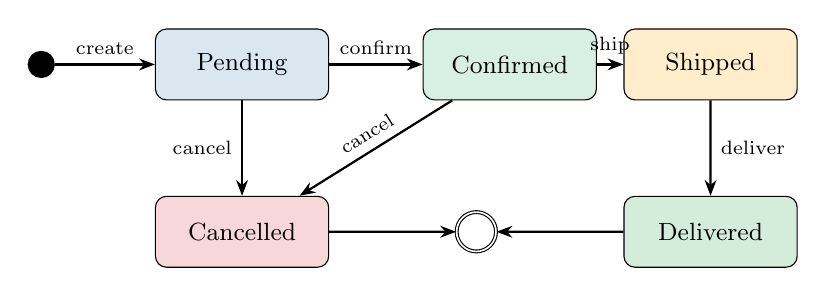
\begin{tikzpicture}[
    scale=0.85,
    state/.style={draw, rounded corners, minimum width=2.2cm, minimum height=0.9cm, font=\small},
    initial/.style={draw, circle, fill=black, minimum size=0.3cm},
    final/.style={draw, circle, double, minimum size=0.5cm},
    trans/.style={-{Stealth[length=2mm]}, thick}
]
    % States
    \node[initial] (start) at (-5,0) {};
    \node[state, fill=componentcolor!20] (pending) at (-2,0) {Pending};
    \node[state, fill=modulecolor!20] (confirmed) at (2,0) {Confirmed};
    \node[state, fill=servicecolor!20] (shipped) at (5,0) {Shipped};
    \node[state, fill=successgreen!20] (delivered) at (5,-2.5) {Delivered};
    \node[state, fill=warningred!20] (cancelled) at (-2,-2.5) {Cancelled};
    \node[final] (end) at (1.5,-2.5) {};
    
    % Transitions
    \draw[trans] (start) -- node[above, font=\scriptsize] {create} (pending);
    \draw[trans] (pending) -- node[above, font=\scriptsize] {confirm} (confirmed);
    \draw[trans] (confirmed) -- node[above, font=\scriptsize] {ship} (shipped);
    \draw[trans] (shipped) -- node[right, font=\scriptsize] {deliver} (delivered);
    \draw[trans] (pending) -- node[left, font=\scriptsize] {cancel} (cancelled);
    \draw[trans] (confirmed) -- node[above, font=\scriptsize, sloped] {cancel} (cancelled);
    \draw[trans] (delivered) -- (end);
    \draw[trans] (cancelled) -- (end);
\end{tikzpicture}
\caption{Order Lifecycle State Machine}
\end{figure}

\begin{longtable}{@{}L{2.2cm} L{3cm} L{3cm} L{4.3cm}@{}}
\caption{Order State Transition Table} \\
\toprule
\textbf{From State} & \textbf{Event/Trigger} & \textbf{To State} & \textbf{Actions/Guards} \\
\midrule
\endfirsthead
\toprule
\textbf{From State} & \textbf{Event/Trigger} & \textbf{To State} & \textbf{Actions/Guards} \\
\midrule
\endhead
\bottomrule
\endlastfoot
(Initial) & CreateOrder & Pending & Validate order; reserve inventory \\
Pending & PaymentSucceeded & Confirmed & Record payment; notify customer \\
Pending & PaymentFailed & Pending & Retry payment; notify if max retries \\
Pending & CancelOrder & Cancelled & Guard: within cancel window; release inventory \\
Confirmed & ShipmentCreated & Shipped & Record tracking; notify customer \\
Confirmed & CancelOrder & Cancelled & Guard: not yet shipped; process refund \\
Shipped & DeliveryConfirmed & Delivered & Record delivery; close order \\
Delivered & (none) & (Final) & Order complete \\
Cancelled & (none) & (Final) & Order terminated \\
\end{longtable}

\subsubsection{State Invariants}

Document properties that must hold true in each state.

\begin{longtable}{@{}L{2.5cm} L{10cm}@{}}
\caption{Order State Invariants} \\
\toprule
\textbf{State} & \textbf{Invariants} \\
\midrule
\endfirsthead
\toprule
\textbf{State} & \textbf{Invariants} \\
\midrule
\endhead
\bottomrule
\endlastfoot
Pending & Inventory reserved; payment not processed; cancel allowed \\
Confirmed & Payment captured; inventory committed; shipment allowed \\
Shipped & Tracking number assigned; delivery pending; cancel not allowed \\
Delivered & Delivery timestamp recorded; all quantities accounted \\
Cancelled & Inventory released; payment refunded (if captured); reason recorded \\
\end{longtable}

\subsection{Behavioral Responsibilities}

Document key algorithms, processing rules, and behavioral contracts.

\begin{tcolorbox}[colback=lightgray, colframe=sectionblue, title=\textbf{Behavioral Specification: Order Total Calculation}]

\textbf{Element:} SVC-ORDER-Process

\textbf{Responsibility:} Calculate accurate order totals

\vspace{0.3cm}
\textbf{Algorithm:}
\begin{enumerate}[nosep]
    \item Sum line item subtotals (quantity $\times$ unit price)
    \item Apply item-level discounts (percentage or fixed)
    \item Calculate subtotal after item discounts
    \item Apply order-level promotions (coupon codes, loyalty points)
    \item Calculate shipping cost based on destination and method
    \item Calculate tax based on shipping destination and product categories
    \item Sum components: subtotal + shipping + tax - order discounts
\end{enumerate}

\vspace{0.3cm}
\textbf{Business Rules:}
\begin{itemize}[nosep]
    \item Maximum one coupon code per order
    \item Loyalty points valued at \$0.01 per point
    \item Tax calculation delegated to tax service for accuracy
    \item Free shipping for orders over \$50 (before tax)
    \item All monetary calculations use banker's rounding
\end{itemize}

\vspace{0.3cm}
\textbf{Preconditions:}
\begin{itemize}[nosep]
    \item All line items have valid product IDs and prices
    \item Shipping address is validated and complete
    \item Customer eligibility for promotions verified
\end{itemize}

\vspace{0.3cm}
\textbf{Postconditions:}
\begin{itemize}[nosep]
    \item Order total equals sum of components (auditable)
    \item All applied discounts recorded with reasons
    \item Tax breakdown recorded by jurisdiction
\end{itemize}

\vspace{0.3cm}
\textbf{Performance:} Calculation completes in $<$ 50ms for orders up to 100 items
\end{tcolorbox}

\subsection{Concurrency and Synchronization}

Document how elements handle concurrent access and maintain consistency.

\begin{longtable}{@{}L{2.5cm} L{3cm} L{7cm}@{}}
\caption{Concurrency Handling} \\
\toprule
\textbf{Element} & \textbf{Mechanism} & \textbf{Description} \\
\midrule
\endfirsthead
\toprule
\textbf{Element} & \textbf{Mechanism} & \textbf{Description} \\
\midrule
\endhead
\bottomrule
\endlastfoot
ORDER-Svc & Optimistic Locking & Version field prevents lost updates; retry on conflict \\
INV-Svc & Database Locks & Row-level locks during reservation; timeout after 5s \\
PAY-Svc & Idempotency Keys & Client-provided keys prevent duplicate charges \\
EVENT-Bus & Partition Keys & Same order always goes to same partition \\
CACHE-Redis & Atomic Operations & SETNX for distributed locks; TTL prevents deadlocks \\
\end{longtable}

\subsection{Failure Modes and Recovery}

Document how elements behave when things go wrong.

\begin{longtable}{@{}L{2.2cm} L{3cm} L{3.5cm} L{3.5cm}@{}}
\caption{Failure Mode Analysis} \\
\toprule
\textbf{Element} & \textbf{Failure Mode} & \textbf{Detection} & \textbf{Recovery} \\
\midrule
\endfirsthead
\toprule
\textbf{Element} & \textbf{Failure Mode} & \textbf{Detection} & \textbf{Recovery} \\
\midrule
\endhead
\bottomrule
\endlastfoot
ORDER-Svc & Database unavailable & Connection timeout & Circuit breaker; queue requests; alert \\
ORDER-Svc & INV-Svc unavailable & gRPC timeout & Degrade to cached inventory; flag for reconciliation \\
ORDER-Svc & PAY-Svc timeout & HTTP 504 & Retry with idempotency key; status: payment\_pending \\
INV-Svc & Oversell detected & Negative stock count & Backorder; notify customer; alert operations \\
PAY-Svc & Gateway rejection & 4xx response & Return error to caller; log for analysis \\
EVENT-Bus & Consumer lag & Lag metric threshold & Scale consumers; alert if lag exceeds SLA \\
\end{longtable}

\subsection{Behavioral References}

Link to detailed behavioral models maintained separately.

\begin{longtable}{@{}L{3cm} L{3.5cm} L{3cm} L{3cm}@{}}
\caption{Behavioral Model References} \\
\toprule
\textbf{Model} & \textbf{Elements Covered} & \textbf{Type} & \textbf{Reference} \\
\midrule
\endfirsthead
\toprule
\textbf{Model} & \textbf{Elements Covered} & \textbf{Type} & \textbf{Reference} \\
\midrule
\endhead
\bottomrule
\endlastfoot
Order Creation Flow & ORDER, INV, PAY & Sequence Diagram & [DOC:seq-order-create] \\
Order Cancellation & ORDER, INV, PAY & Sequence Diagram & [DOC:seq-order-cancel] \\
Saga: Order Fulfillment & ORDER, INV, PAY, FULFILL & Saga Diagram & [DOC:saga-fulfillment] \\
Inventory Reservation & INV-Svc & State Machine & [DOC:state-inventory] \\
Payment Processing & PAY-Svc & Activity Diagram & [DOC:activity-payment] \\
Authentication Flow & USER-Auth & Sequence Diagram & [DOC:seq-auth-flow] \\
\end{longtable}

%==============================================================================
\section{Traceability and Cross-References}
%==============================================================================

\subsection{Traceability Framework}

Traceability connects catalog elements to other artifacts, enabling impact analysis, compliance verification, and knowledge navigation.

\begin{figure}[H]
\centering
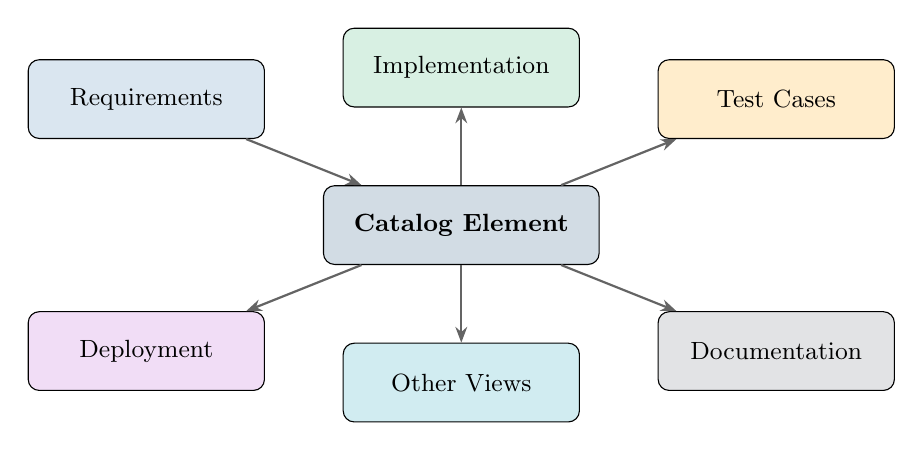
\begin{tikzpicture}[
    scale=0.8,
    box/.style={draw, rounded corners, minimum width=3cm, minimum height=1cm, font=\small, align=center},
    arrow/.style={-{Stealth[length=2mm]}, thick, flowcolor}
]
    % Central element
    \node[box, fill=sectionblue!20, minimum width=3.5cm] (element) at (0,0) {\textbf{Catalog Element}};
    
    % Connected artifacts
    \node[box, fill=componentcolor!20] (req) at (-5,2) {Requirements};
    \node[box, fill=modulecolor!20] (impl) at (0,2.5) {Implementation};
    \node[box, fill=servicecolor!20] (test) at (5,2) {Test Cases};
    \node[box, fill=datacolor!20] (deploy) at (-5,-2) {Deployment};
    \node[box, fill=infoblue!20] (views) at (0,-2.5) {Other Views};
    \node[box, fill=lowgray!20] (docs) at (5,-2) {Documentation};
    
    % Arrows
    \draw[arrow] (req) -- (element);
    \draw[arrow] (element) -- (impl);
    \draw[arrow] (element) -- (test);
    \draw[arrow] (element) -- (deploy);
    \draw[arrow] (element) -- (views);
    \draw[arrow] (element) -- (docs);
\end{tikzpicture}
\caption{Element Traceability Relationships}
\end{figure}

\subsection{Requirements Traceability}

Map elements to the requirements they satisfy.

\begin{longtable}{@{}L{2.5cm} L{5cm} L{5cm}@{}}
\caption{Requirements Traceability Matrix} \\
\toprule
\textbf{Element} & \textbf{Functional Requirements} & \textbf{Non-Functional Requirements} \\
\midrule
\endfirsthead
\toprule
\textbf{Element} & \textbf{Functional Requirements} & \textbf{Non-Functional Requirements} \\
\midrule
\endhead
\bottomrule
\endlastfoot
ORDER-Svc & FR-ORD-001 through FR-ORD-050 & NFR-PERF-01, NFR-AVAIL-01, NFR-SEC-03 \\
INV-Svc & FR-INV-001 through FR-INV-025 & NFR-PERF-02, NFR-AVAIL-02 \\
PAY-Svc & FR-PAY-001 through FR-PAY-030 & NFR-SEC-01, NFR-SEC-02, NFR-COMPL-01 \\
USER-Auth & FR-AUTH-001 through FR-AUTH-020 & NFR-SEC-04, NFR-PERF-03 \\
EVENT-Bus & FR-EVT-001 through FR-EVT-010 & NFR-REL-01, NFR-SCAL-01 \\
\end{longtable}

\subsection{Implementation Mapping}

Map elements to source code and deployment artifacts.

\begin{longtable}{@{}L{2.5cm} L{4cm} L{3cm} L{3cm}@{}}
\caption{Implementation Artifact Mapping} \\
\toprule
\textbf{Element} & \textbf{Source Repository} & \textbf{Package/Module} & \textbf{Artifact} \\
\midrule
\endfirsthead
\toprule
\textbf{Element} & \textbf{Source Repository} & \textbf{Package/Module} & \textbf{Artifact} \\
\midrule
\endhead
\bottomrule
\endlastfoot
ORDER-Svc & github.com/co/order-service & com.company.order & order-service.jar \\
INV-Svc & github.com/co/inventory-svc & inventory & inventory-svc (Go binary) \\
PAY-Svc & github.com/co/payment-svc & com.company.payment & payment-service.jar \\
USER-Auth & github.com/co/auth-service & auth & auth-service (Go binary) \\
API-Gateway & github.com/co/api-gateway & api-gateway & Docker: api-gateway \\
\end{longtable}

\subsection{Cross-View References}

Map elements to their appearances in other architectural views.

\begin{longtable}{@{}L{2.5cm} L{3cm} L{3cm} L{4cm}@{}}
\caption{Cross-View Element Mapping} \\
\toprule
\textbf{Element} & \textbf{This View} & \textbf{Other View} & \textbf{Representation} \\
\midrule
\endfirsthead
\toprule
\textbf{Element} & \textbf{This View} & \textbf{Other View} & \textbf{Representation} \\
\midrule
\endhead
\bottomrule
\endlastfoot
ORDER-Svc & Component-Connector & Module View & order-service module \\
ORDER-Svc & Component-Connector & Deployment View & order-svc-cluster pod \\
ORDER-Svc & Component-Connector & Data Flow View & Order Processing process \\
ORDER-DB & Component-Connector & Deployment View & orders-db-primary node \\
EVENT-Bus & Component-Connector & Deployment View & kafka-cluster \\
\end{longtable}

\subsection{Decision Traceability}

Link elements to architectural decisions that shaped them.

\begin{longtable}{@{}L{2.5cm} L{2cm} L{8cm}@{}}
\caption{Architectural Decision References} \\
\toprule
\textbf{Element} & \textbf{ADR ID} & \textbf{Decision Summary} \\
\midrule
\endfirsthead
\toprule
\textbf{Element} & \textbf{ADR ID} & \textbf{Decision Summary} \\
\midrule
\endhead
\bottomrule
\endlastfoot
ORDER-Svc & ADR-005 & Use saga pattern for distributed transactions \\
EVENT-Bus & ADR-008 & Adopt Apache Kafka for event streaming \\
PAY-Svc & ADR-012 & Isolate payment processing for PCI compliance \\
USER-Auth & ADR-003 & Implement OAuth 2.0 with JWT tokens \\
All Services & ADR-001 & Adopt microservices architecture \\
All Services & ADR-015 & Use gRPC for internal service communication \\
\end{longtable}

%==============================================================================
\section{Catalog Governance and Maintenance}
%==============================================================================

\subsection{Ownership and Accountability}

Each element should have clear ownership for maintenance and evolution.

\begin{longtable}{@{}L{2.5cm} L{3cm} L{3cm} L{4cm}@{}}
\caption{Element Ownership Registry} \\
\toprule
\textbf{Element} & \textbf{Owning Team} & \textbf{Technical Owner} & \textbf{Contact} \\
\midrule
\endfirsthead
\toprule
\textbf{Element} & \textbf{Owning Team} & \textbf{Technical Owner} & \textbf{Contact} \\
\midrule
\endhead
\bottomrule
\endlastfoot
ORDER-Svc & Order Team & J. Smith & order-team@company.com \\
INV-Svc & Inventory Team & A. Jones & inventory-team@company.com \\
PAY-Svc & Payments Team & B. Chen & payments-team@company.com \\
USER-Auth & Platform Team & M. Garcia & platform-team@company.com \\
API-Gateway & Platform Team & M. Garcia & platform-team@company.com \\
EVENT-Bus & Platform Team & K. Patel & platform-team@company.com \\
\end{longtable}

\subsection{Change Management Process}

Changes to catalog entries should follow a controlled process.

\begin{enumerate}
    \item \textbf{Propose:} Submit change request with rationale and impact analysis
    \item \textbf{Review:} Architecture review board evaluates change
    \item \textbf{Approve:} Obtain approval from element owner and affected stakeholders
    \item \textbf{Implement:} Update catalog entry with version increment
    \item \textbf{Validate:} Verify catalog matches implementation
    \item \textbf{Communicate:} Notify dependent teams of changes
\end{enumerate}

\subsection{Quality Assurance}

Maintain catalog quality through regular validation.

\begin{bestpractice}
\textbf{Catalog Quality Checklist:}
\begin{itemize}[nosep]
    \item All elements in diagrams have catalog entries
    \item All catalog entries correspond to actual elements
    \item No orphan elements (in catalog but not in any diagram)
    \item No phantom elements (in diagram but not in catalog)
    \item Interface specifications match implementation
    \item Cross-references are valid and current
    \item Version information is accurate
    \item Ownership information is current
\end{itemize}
\end{bestpractice}

\subsection{Catalog Version History}

\begin{longtable}{@{}L{1.5cm} L{2cm} L{2.5cm} L{6.5cm}@{}}
\caption{Catalog Version History} \\
\toprule
\textbf{Version} & \textbf{Date} & \textbf{Author} & \textbf{Changes} \\
\midrule
\endfirsthead
\toprule
\textbf{Version} & \textbf{Date} & \textbf{Author} & \textbf{Changes} \\
\midrule
\endhead
\bottomrule
\endlastfoot
1.0.0 & 2024-01-15 & Architecture Team & Initial catalog creation \\
1.1.0 & 2024-02-20 & J. Smith & Added ORDER-Svc behavioral specifications \\
1.2.0 & 2024-03-15 & A. Jones & Updated INV-Svc interface documentation \\
1.3.0 & 2024-04-10 & B. Chen & Added PAY-Svc v2 interface specifications \\
2.0.0 & 2024-06-01 & Architecture Team & Major revision; added EVENT-Bus; updated all interfaces \\
\end{longtable}

%==============================================================================
\section{Common Pitfalls and Anti-patterns}
%==============================================================================

\begin{warning}
\textbf{Avoid These Catalog Anti-patterns:}

\textbf{Stale Catalog:} Catalog that doesn't match current implementation. Establish automated validation where possible.

\textbf{Over-Documentation:} Excessive detail that becomes unmaintainable. Document what's needed, not everything possible.

\textbf{Under-Documentation:} Missing critical information like interface contracts or quality requirements. Use checklists to ensure completeness.

\textbf{Inconsistent Abstraction:} Mixing high-level and low-level elements. Maintain consistent abstraction within each view.

\textbf{Missing Relationships:} Documenting elements but not their relationships. Relationships are as important as elements.

\textbf{Orphan Interfaces:} Interface specifications without corresponding element documentation.

\textbf{Copy-Paste Errors:} Duplicated content that becomes inconsistent. Use single-source references where possible.

\textbf{Unclear Ownership:} No one responsible for keeping entries current. Assign and enforce ownership.
\end{warning}

%==============================================================================
\section{Appendix A: Element Specification Templates}
%==============================================================================

\subsection{Service Element Template}

\begin{tcolorbox}[colback=white, colframe=flowcolor]
\textbf{Service Element Specification}

\vspace{0.2cm}
\textbf{Identity}
\begin{itemize}[nosep]
    \item ID: \rule{5cm}{0.4pt}
    \item Name: \rule{5cm}{0.4pt}
    \item Version: \rule{2cm}{0.4pt}
    \item Stereotype: \rule{3cm}{0.4pt}
\end{itemize}

\vspace{0.2cm}
\textbf{Purpose:} \rule{10cm}{0.4pt}

\vspace{0.2cm}
\textbf{Responsibilities:}
\begin{itemize}[nosep]
    \item \rule{10cm}{0.4pt}
    \item \rule{10cm}{0.4pt}
    \item \rule{10cm}{0.4pt}
\end{itemize}

\vspace{0.2cm}
\textbf{Properties}
\begin{itemize}[nosep]
    \item Criticality: \rule{3cm}{0.4pt}
    \item Availability: \rule{3cm}{0.4pt}
    \item Performance: \rule{5cm}{0.4pt}
    \item Technology: \rule{5cm}{0.4pt}
\end{itemize}

\vspace{0.2cm}
\textbf{Provided Interfaces:} \rule{8cm}{0.4pt}

\vspace{0.2cm}
\textbf{Required Interfaces:} \rule{8cm}{0.4pt}

\vspace{0.2cm}
\textbf{Traceability}
\begin{itemize}[nosep]
    \item Requirements: \rule{6cm}{0.4pt}
    \item Implementation: \rule{6cm}{0.4pt}
\end{itemize}
\end{tcolorbox}

\subsection{Data Store Element Template}

\begin{tcolorbox}[colback=white, colframe=flowcolor]
\textbf{Data Store Element Specification}

\vspace{0.2cm}
\textbf{Identity}
\begin{itemize}[nosep]
    \item ID: \rule{5cm}{0.4pt}
    \item Name: \rule{5cm}{0.4pt}
    \item Type: \rule{3cm}{0.4pt} (Relational / Document / Key-Value / Graph)
\end{itemize}

\vspace{0.2cm}
\textbf{Purpose:} \rule{10cm}{0.4pt}

\vspace{0.2cm}
\textbf{Data Characteristics}
\begin{itemize}[nosep]
    \item Primary Entities: \rule{6cm}{0.4pt}
    \item Volume: \rule{4cm}{0.4pt}
    \item Growth Rate: \rule{4cm}{0.4pt}
    \item Retention: \rule{4cm}{0.4pt}
\end{itemize}

\vspace{0.2cm}
\textbf{Access Patterns}
\begin{itemize}[nosep]
    \item Read/Write Ratio: \rule{3cm}{0.4pt}
    \item Query Complexity: \rule{4cm}{0.4pt}
    \item Throughput: \rule{4cm}{0.4pt}
\end{itemize}

\vspace{0.2cm}
\textbf{Properties}
\begin{itemize}[nosep]
    \item Criticality: \rule{3cm}{0.4pt}
    \item Consistency: \rule{3cm}{0.4pt} (Strong / Eventual)
    \item Backup/Recovery: \rule{5cm}{0.4pt}
    \item Technology: \rule{5cm}{0.4pt}
\end{itemize}
\end{tcolorbox}

%==============================================================================
\section{Appendix B: Glossary}
%==============================================================================

\begin{description}[leftmargin=3cm, style=nextline]
    \item[Architectural Element] A fundamental building block of software architecture with defined interfaces and responsibilities
    \item[Catalog] A structured collection of element specifications within an architectural view
    \item[Component] A modular, deployable unit of software with explicit interfaces
    \item[Connector] An architectural element that mediates interaction between components
    \item[Interface] A defined boundary through which elements interact, specifying operations, data, and protocols
    \item[Module] A code unit implementing a coherent set of responsibilities
    \item[Property] A measurable or classifiable characteristic of an element
    \item[Relation] A connection or dependency between architectural elements
    \item[Service] An independently deployable unit providing capabilities through well-defined interfaces
    \item[Stereotype] A classification tag indicating an element's pattern or role
    \item[Traceability] The ability to relate architectural elements to other artifacts
    \item[View] A representation of a system from a particular perspective
\end{description}

%==============================================================================
\section{Appendix C: References}
%==============================================================================

\begin{enumerate}
    \item Clements, P., et al. (2010). \textit{Documenting Software Architectures: Views and Beyond} (2nd ed.). Addison-Wesley.
    
    \item Bass, L., Clements, P., \& Kazman, R. (2021). \textit{Software Architecture in Practice} (4th ed.). Addison-Wesley.
    
    \item IEEE. (2011). \textit{ISO/IEC/IEEE 42010:2011 Systems and Software Engineering---Architecture Description}.
    
    \item Brown, S. (2018). \textit{The C4 Model for Visualising Software Architecture}. Retrieved from \url{https://c4model.com}
    
    \item Fowler, M. (2002). \textit{Patterns of Enterprise Application Architecture}. Addison-Wesley.
    
    \item Richardson, C. (2018). \textit{Microservices Patterns}. Manning Publications.
    
    \item Vernon, V. (2013). \textit{Implementing Domain-Driven Design}. Addison-Wesley.
    
    \item The Open Group. (2019). \textit{ArchiMate 3.1 Specification}. Van Haren Publishing.
\end{enumerate}

\end{document}